\documentclass[ngerman]{scrartcl} 

\KOMAoptions{fontsize=12pt, paper=a4}
\KOMAoptions{DIV=11}
\usepackage[utf8]{inputenc}             % Direkte Eingabe von ä usw.
\usepackage[T1]{fontenc}               	% Font Kodierung für die Ausgabe
\usepackage{babel}                   	% Verschiedenste sprach-spezifische Extras
\usepackage[autostyle=true]{csquotes}	% Intelligente Anführungszeichen
\usepackage{amsmath}					% Mathematischer Formelsatz mit zusaetzlichen mathematischen Schriften und Symbolen
\usepackage{amssymb}					% Mathematischer Formelsatz mit zusaetzlichen mathematischen Schriften und Symbolen
\usepackage{physics}					% Differentialgleichungen
\usepackage{listings}					% Zum Einbinden von Programmcode verwenden wir das listings-Paket
\usepackage[dvipsnames]{xcolor}			% um Elemente von Befehlen farblich zu unterstützen
\usepackage[varg]{txfonts}              % Schönere Schriftart
\usepackage{graphicx}					% Paket um externe Graphiken einzufuegen
\RequirePackage[backend=biber, style=numeric]{biblatex} % Literaturverzeichnis
\usepackage{hyperref} 					% um klickbare Elemente in Ihrem PDF-Ausgabedokument zu erzeugen
\RequirePackage[all]{hypcap} 			% ergänzend zu hyperref
\usepackage{siunitx}					% Intelligentes Setzten von Zahlen und Einheiten
\usepackage{enumitem}					% Aufzählungsarten
\usepackage{fancyhdr}

\setlength\parindent{0pt} 				% Sets paragraph indentation to 0

\lstset{									% Deutsche Umlaute
	basicstyle=\ttfamily,    
	literate={~} {$\sim$}{1} 				% set tilde as a literal
	{ö}{{\"o}}1
	{ä}{{\"a}}1
	{ü}{{\"u}}1
	{ß}{{\ss}}1
	{Ö}{{\"O}}1
	{Ä}{{\"A}}1
	{Ü}{{\"U}}1
}
\lstset{
	numbers=left, 						% Line numbering
	numberstyle=\footnotesize, 			% Size of numbers
	basicstyle=\ttfamily\small, 		% Style and Size of Text
	backgroundcolor=\color{White}, 		% Background Color
	language=Python, 					% Language of Code
	commentstyle=\color{Maroon}, 		% Color and Style of Comments
	stringstyle=\color{OliveGreen}, 	% Color of Strings
	showstringspaces=false,
	morekeywords={import,from,class,def,for,while,if,is,in,elif,else,not,and,or,print,break,continue,return,True,False,None,access,as,del,except,exec,finally,global,import,lambda,pass,print,raise,try,assert}, 									% Definition of new keywords that will be highlighted
	keywordstyle=\color{RoyalBlue}		% Color and Style of Keywords
}


\pagestyle{fancy}
\fancyhf{}
\rhead{Lukas Sabatschus, Ruth Jacobs}
\lhead{Computerphysik - Abgabe 3}
\rfoot{Seite \thepage}

\title{Computerphysik - Abgabe 3}
\date{\today}

\begin{document}
% Auf 3 setzen, da es beim ersten Chapter um 1 hochgezählt wird. 3+1=4
\setcounter{section}{6}
\thispagestyle{fancy}

\section{Eigenwerte linearer Differentialoperatoren}
\subsection{}
Für eine Lösung des inhomogenen Systems können beliebige Linearkombinationen von Lösungen
des homogenen Systems hinzuaddiert werden, um neue Lösungen des imhomogenen Systems zu bekommen.
Sei $h(x)$ eine Lösung des homogenen Systems und $u(x)$ eine Lösung des inhomogenen Systems gilt:
\begin{align*}
	Dh(x)-\lambda h(x)&=0\\
	Du(x)-\lambda u(x)&=f(x)\\
	g(x) &:= u(x)+a*h(x)\\
	\Rightarrow Dg(x)-\lambda g(x) &= f(x)+a*0\\
	g(t_{0,1}) &= u(t_{0,1})+a*f(t_{0,1}) = u(t_{0,1}) 
\end{align*}
Also ist $g(x)$ eine Lösung des inhomogenen Systems.


\subsection{}
In dieser Teilaufgabe geht es darum die Eigenwerte der homogenen Differentialgleichung: $Du = u'' + gu$ zu bestimmen mit $g \equiv 0$. Deshalb gilt mit der Eigenwertgleichung:\\ $ D u_{\lambda} - \lambda u_{\lambda} = 0$:
\begin{equation*}
	u_{\lambda}'' - \lambda u_{\lambda} = 0
\end{equation*}

Nun wird das Numerov-Verfahren genutzt um diese DGL mit den Randbedingungen $u(0)=1$ und $u(60)=1$ zu lösen. \\
Dafür wird $\lambda$ variiert und jeweils die Lösung $u$ bestimmt, indem man die Anfangssteigung der Funktion im Punkt P(60|0) solange verändert, bis die Funktion die andere Randbedingung erfüllt. Die Lösungsfunktionen $u$ haben nun verscheidene Amplituden und man kann feststellen, dass für bestimmte $\lambda$ die Amplituden gegen $\infty$ gehen.\\
Dies liegt darin begründet, dass für manche $\lambda$ die Funktion durch den Punkt Q(0|0) läuft und damit beliebig skaliert werden kann, den Punkt (0|1), der durch das Randwertproblem vorgegeben ist aber nie erreicht. Wenn wir nun die Amplituden der Funktionen $u$ gegen $\lambda$ auftragen, können wir erkennen, dass die Amplitude an verschiedenen Stellen gegen $\infty$ läuft. Dies müssen dann die Lösungen der homogenen DGL mit homogenen Randbedingungen sein. Die Werte der ersten 10 Eigenwerte sind:

\begin{tabular}[h]{l|l}
	Anzahl & Eigenwert \\
	\hline
	1& -0.274000\\
	2& -0.222000\\
	3& -0.175400\\
	4& -0.134200\\
	5& -0.098600\\
	6& -0.068400\\
	7& -0.043800\\
	8& -0.024600\\
	9& -0.010900\\
	10& -0.002600 \\
\end{tabular}\\

\begin{figure}[htbp]
	\centering
	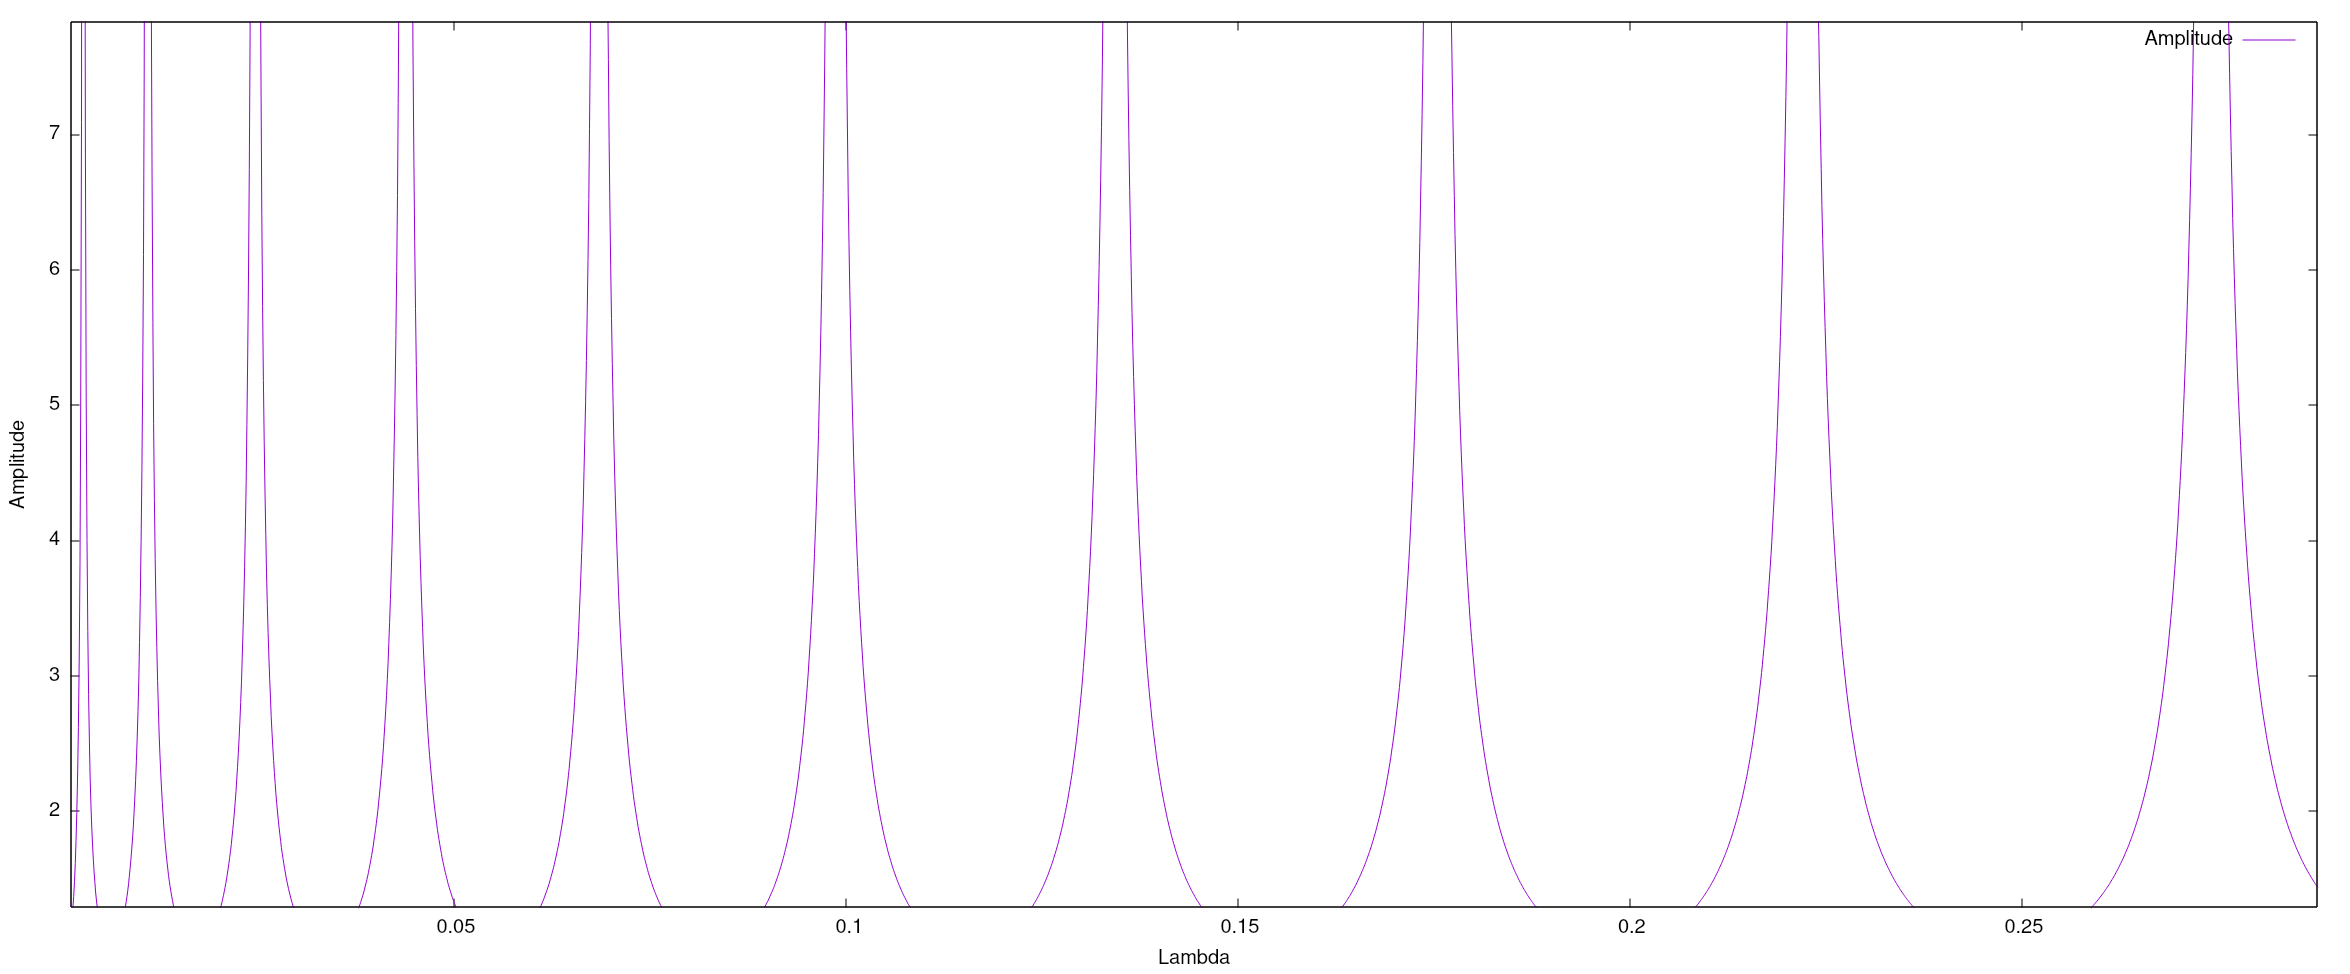
\includegraphics[width=0.95\textwidth]{H7}
	\caption[Bestimmung Eigenwerte]{Bestimmung der Eigenwerte}
	\label{fig:7.1}
\end{figure}

was sich auch in Abbildung \ref{fig:7.1} erkennen lässt.
Das Programm für diese Aufgabe ist als \emph{H7.c} zu finden

Nun kann man die numerisch bestimmten Eigenwerte noch mit den analytisch berechneten vergleichen. Die analytische Lösung lautet:

\begin{align*}
	u''=\lambda u 	
\end{align*}

mit $u(60)=0 \equiv u_0$ und $u(0)=0 \equiv u_1$

Damit sind die Werte im Vergleich

%Tabelle




\section{Kronig-Penney Model}
Wir suchen das $\lambda$, welches genau beide Randbedingungen erfüllt, indem wir das Sekantenverfahren auf den Abstand der Nullstelle von der Randbedingung anwenden.

Nullstelle 1 bei 25.394003
Nullstelle 2 bei 25.419690
Nullstelle 3 bei 25.457850
Nullstelle 4 bei 25.502437
Nullstelle 5 bei 25.546573
Nullstelle 6 bei 25.583643
Nullstelle 7 bei 25.608240
\end{document}







